\documentclass[a4paper]{article}

\usepackage[utf8x]{inputenc}

\usepackage[left=1cm,top=2cm,right=1cm,bottom=2cm]{geometry}

\usepackage{geometry}
\geometry{a4paper}

\usepackage{graphicx}

\usepackage{minted}
% global minted style  
\setminted{  
encoding=utf-8
}

\usepackage{fancyhdr}

\pagestyle{fancy}
\fancyhf{}
\rhead{Palvinder Sander}
\lhead{Machine Learning Assessment One}
\rfoot{Page \thepage}

\usepackage{mathpartir}

\usepackage{bussproofs}
\usepackage{cancel}
\usepackage{tabularx}

%\usepackage{tcolorbox}
%\usepackage{etoolbox}
%\BeforeBeginEnvironment{minted}{\begin{tcolorbox}}%
%\AfterEndEnvironment{minted}{\end{tcolorbox}}%

\title{Logic Assessment One}
\author{Palvinder Sander}
\date{}

\begin{document}

\section*{Question One:}

Univariate non-linear regression in Java with inital values of $w_{0}$, $w_{1}$ and $w_{2}$ set to $0$ and $\alpha$ set to $0.00000001$ over $100$ epochs.

%\inputminted[frame=single,framesep=10pt,mathescape=true,escapeinside=||]{java}{nonLinearReg.java}

\noindent My code\footnote{solution1.java} yields the following output:

\begin{minted}[frame=single,framesep=10pt,mathescape=true,escapeinside=||]{java}
h(x) = (0.10000515906009057 * x^2) + (-5.183013415310536E-4 * x) + 1.7778308805231613E-4
\end{minted}

\noindent After plotting this function (using xchart) we can see parameterized hypothesis function fits the training data relatively well.

\begin{figure}[h]
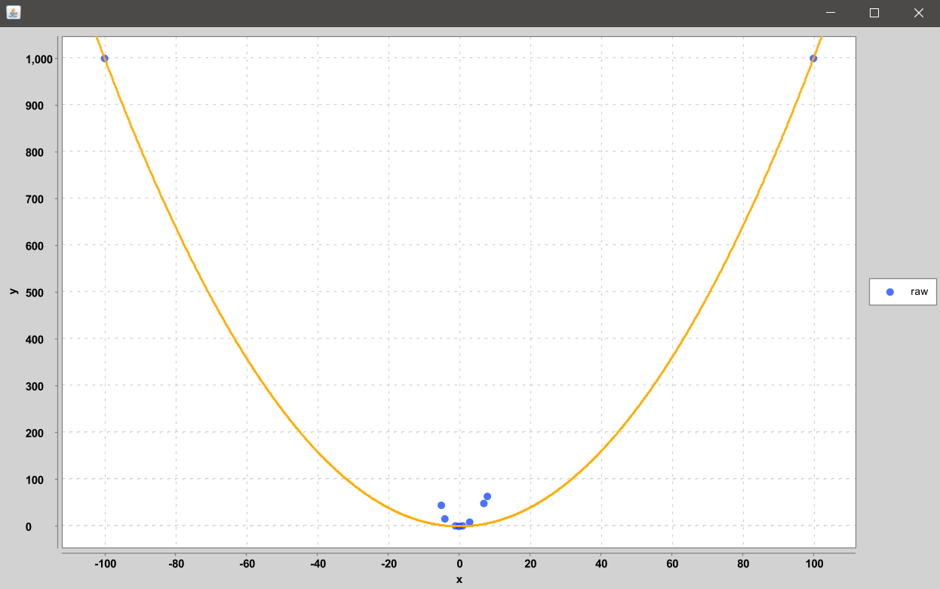
\includegraphics[scale=1]{q1.png}
\centering
\end{figure}
lol
\end{document}